% -------------- TABLA PARA REQUERIMIENTOS FUNCIONALES ---------------- %
% Nomenclatura para la prioridad:
%	MA - Muy Alta
%	A - Alta
%	M - Media
%	B - Baja
%	MB - Muy Baja

\begin{table}[htbp!]
    \begin{requerimientos}

        \FRitem{RM1}{Gestionar Unidad de Aprendizaje}{El sistema debe permitirle al usuario Docente gestionar de las Unidades de Aprendizaje que contiene el Mapa Curricular.}{A}{Origen}
        \label{RM1}

        \FRitem{RM2}{Gestionar Usuarios de la Unidad Académica}{El sistema debe permitirle al Jefe de Innovación Educativa de  la gestión de los usuarios integrantes de la Unidad Académica (Analista y Docente).}{A}{Origen}
        \label{RM2}

        \FRitem{RM3}{Finalizar Carga Mapa Curricular}{El sistema debe permitirle al usuario Docente indicar cuando ya a finalizado el registro de todas las Unidades de Aprendizaje que contiene el Mapa  Curricular.}{A}{Origen}
        \label{RM3}

        \FRitem{RM4}{Guardar Avances del Mapa Curricular}{El sistema debe permitirle al usuario Docente guardar las Unidades de Aprendizaje que que este vaya registrando.}{M}{Origen}
        \label{RM4}

        \FRitem{RM5}{Consultar Mapa Curricular }{El sistema debe permitirle al usuario Docente visualizar la totalidad de los contenidos del Mapa Curricular registrados.}{M}{Origen}
        \label{RM5}

        \FRitem{RM6}{Validar congruencia en el Mapa Curricular}{ El Sistema validará la congruencia de los datos registrados.}{M}{Origen}
        \label{RM6}

        \FRitem{RM7}{Aprobar Mapa Curricular}{el Sistema debe permitirle al Usuario Jefe  de Innovación Educativa aprobar el Mapa Curricular una vez que el registro haya finalizado.}{M}{Origen}
        \label{RM7}

        \FRitem{RM8}{Enviar Comentarios}{ El Sistema debe permitirle a los Usuarios del Departamento de Innovación Educativa enviar comentarios de corrección sobre el Mapa Curricular una vez que el registro haya finalizado.}{M}{Origen}
        \label{RM8}

        \FRitem{RM9}{Visualizar Comentarios}{ El Sistema debe permitirle al Usuario Docente visualizar comentarios hechos al Mapa Curricular, tanto por el Departamento de Innovación Educativa como por la DES.}{M}{Origen}
        \label{RM9}

        \FRitem{RM10}{Revisar Mapa Curricular}{el Sistema debe permitirle al Usuario Analista revisar el Mapa Curricular una vez que el registro haya finalizado.}{B}{Origen}
        \label{RM10}
    \end{requerimientos}
    \caption{Requerimientos funcionales del sistema para el subproceso de elaboración del Mapa Curricular}
    \label{tbl:RFUA}
\end{table}

\begin{figure}[htbp]
    \begin{center}
        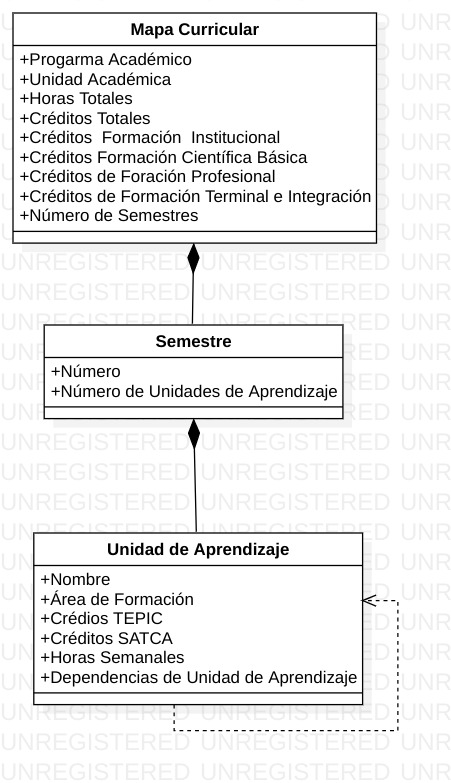
\includegraphics[width=.50\textwidth]{C2-DR/SP4/Image/ModeloDeDatosMC}
        \label{MD-SP4}
        \caption{Modelo de Datos Subproceso para la  Carga del Mapa Curricular}
    \end{center}
\end{figure}

\begin{figure}[htbp]
	\begin{center}
		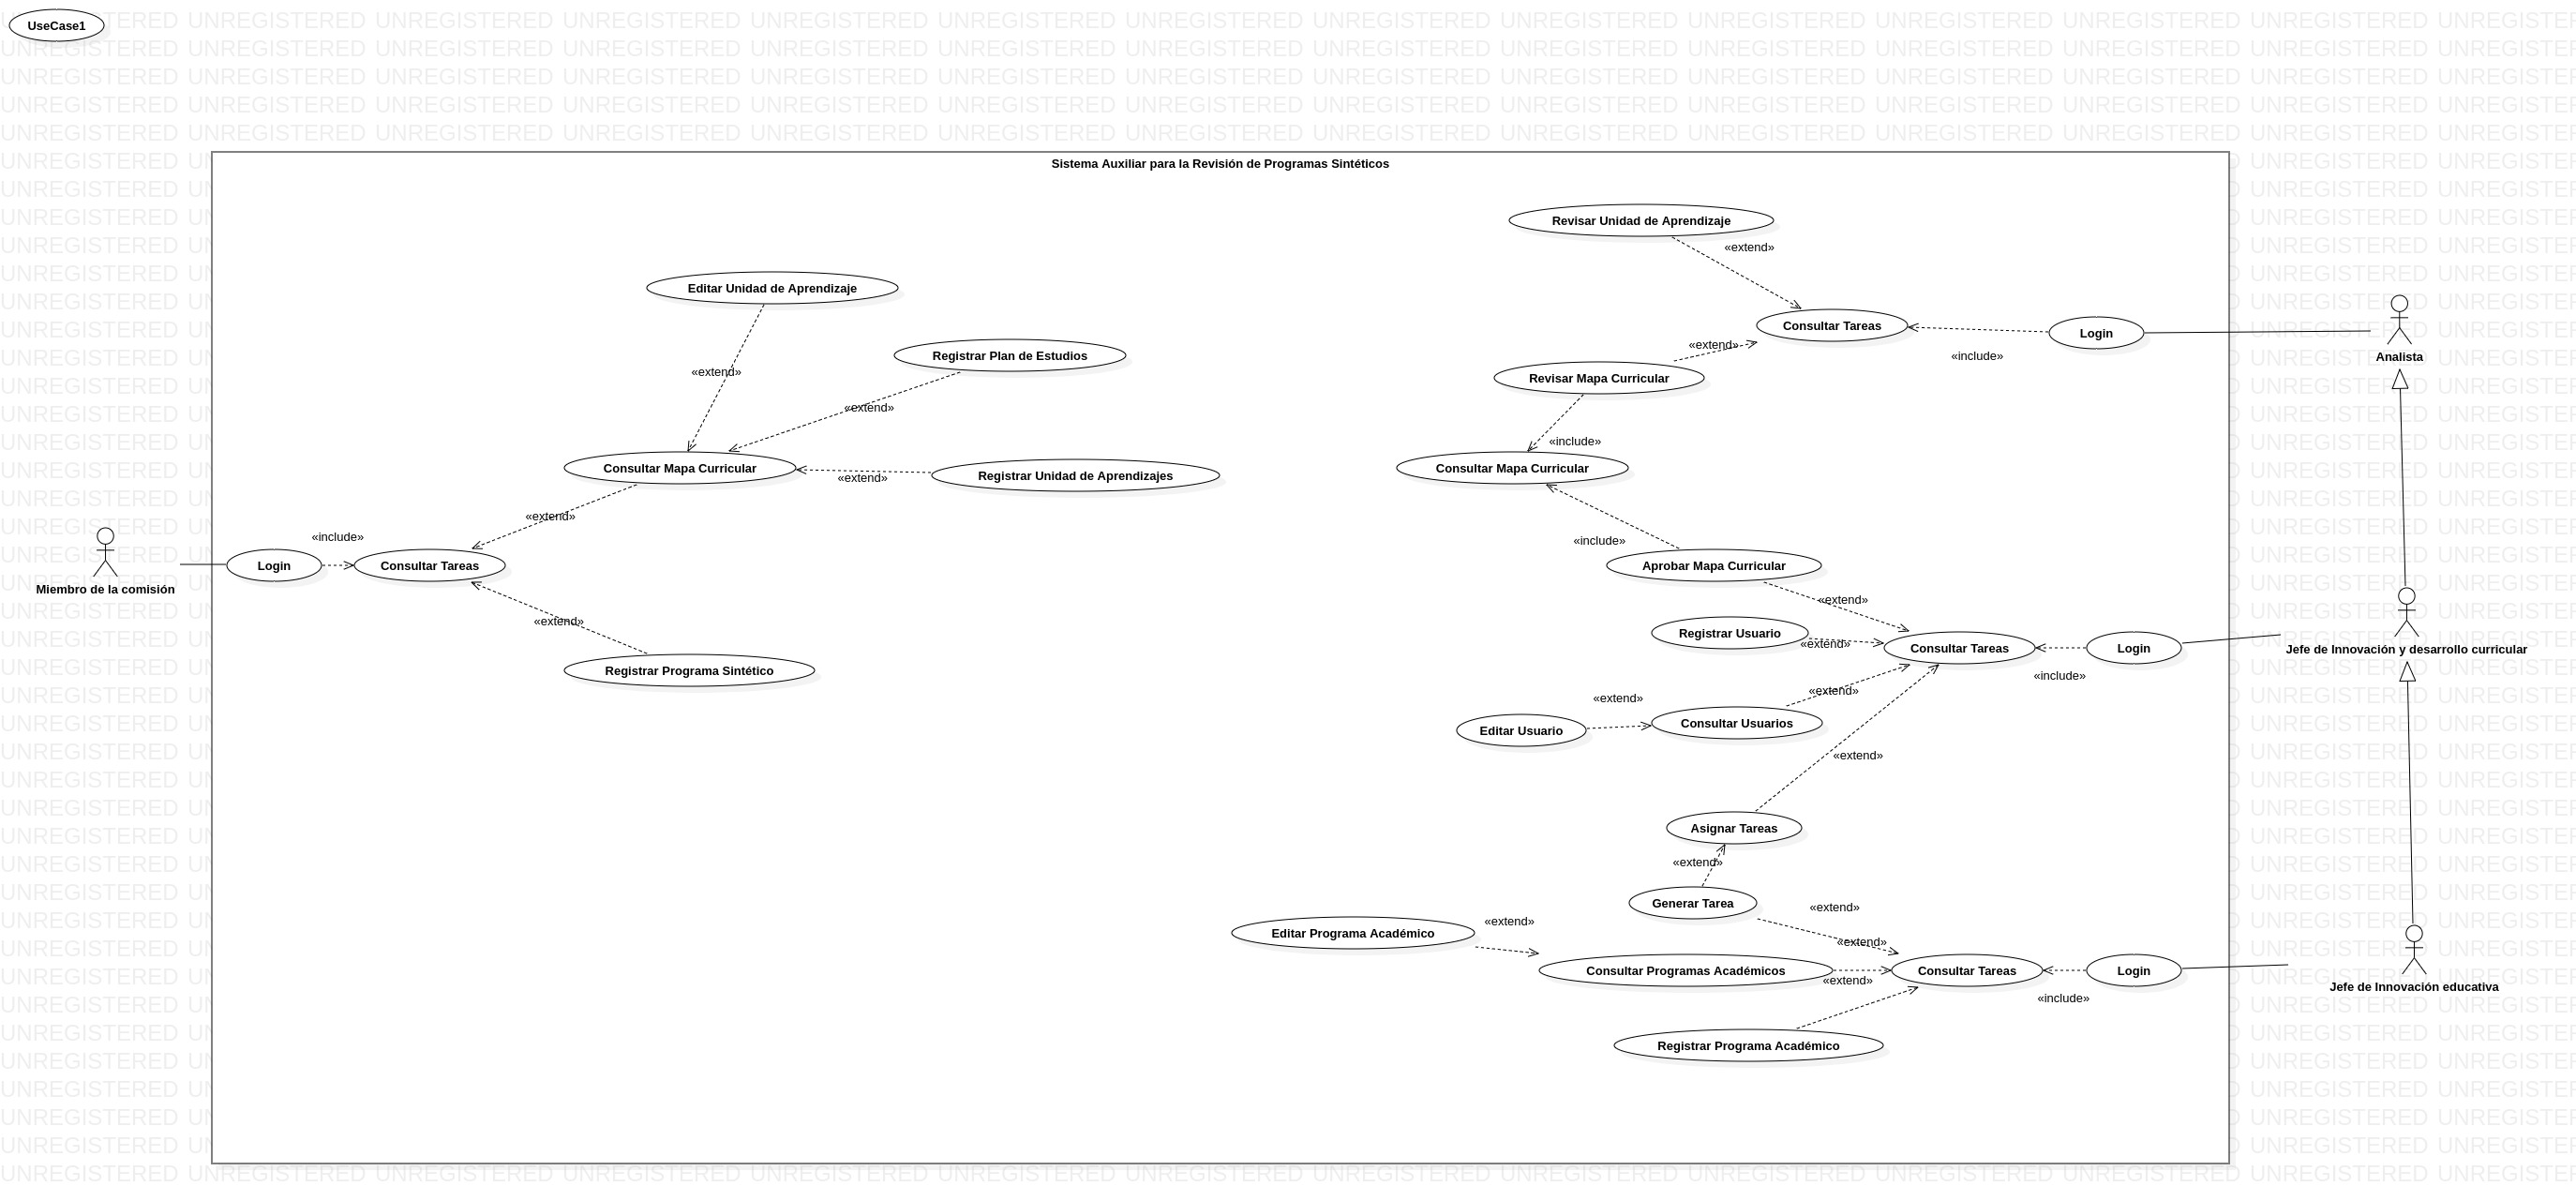
\includegraphics[width=.95\textwidth]{C2-DR/SP4/Image/CasosDeUso}
		\caption{Casos de Uso Subproceso para la  Carga del Mapa Curricular}
		\label{CU-SP4}
	\end{center}
\end{figure}

\begin{center}
	\begin{tabular}{|c|c|c|c|}
		\hline
		ID & Caso de uso & Requerimientos & Encargado \\ \hline
        1 & Registrar Mapa Curricular & \hyperref[RM1]{RM1} & Josué \\ \hline
        2 & Guardar Mapa Curricular & \hyperref[RM4]{RM4} & Andrés \\ \hline
        3 & Consultar Mapa Curricular & \hyperref[RM5]{RM5} & Arturo \\ \hline
		4 & Editar Información General & \hyperref[RM6]{RM6} & Josué \\ \hline
        5 & Finalizar Mapa Curricular & \hyperref[RM3]{RM3} & Josué \\ \hline
        6 & Aprobar Mapa Curricular & \hyperref[RM11]{RM11} & Andrés \\ \hline
        7 & Registrar Unidades de Aprendizaje & \hyperref[RM2]{RM2} & Arturo \\ \hline
        8 & Editar Unidades de Aprendizaje & \hyperref[RM8]{RM8} & Andrés \\ \hline
        9 & Eliminar Unidades de Aprendizaje & \hyperref[RM7]{RM7} & Arturo \\ \hline
        10 & Registrar Dependencias & \hyperref[RM9]{RM9} & Andrés \\ \hline
        11 & Editar Dependencias & \hyperref[RM9]{RM9} & Josué \\ \hline
        12 & Eliminar Dependencias & \hyperref[RM9]{RM9} & Arturo \\ \hline
        13 & Visualizar Comentarios & \hyperref[RM13]{RM13} & Josué \\ \hline
        14 & Enviar Comentarios & \hyperref[RM12]{RM12} & Andrés \\ \hline
    \end{tabular}
\end{center}
